\appendix
\begin{appendices}
\chapter{Begriffe}
\section*{A...}
\begin{description}
\item[Adresse] \enquote{Nummer des Bytes im Speicher}, ab dem eine Information zu finden ist.\newline
	Siehe Abschnitt \ref{sec:Pointer}
\item[Adress-Operator] Das Zeichen \texttt{\&}. Wird vor Variablen gestellt, um den Speicherort (\ie die 
	\emph{Adresse}) der Variable zu ermitteln.\newline
	Siehe Abschnitt \ref{sec:Pointer}
\item[Allozieren] Anfrage an das Betriebssystem, einen Speicherbereich für andere Programme zu sperren,
	also den Speicherbereich für eine bestimmte Aufgabe zu \emph{reservieren}. Üblicherweise mit den 
	Befehlen \texttt{malloc} oder \texttt{calloc} aus dem \emph{Header} \texttt{<stdlib.h>} umgesetzt.
	\newline
	Siehe Abschnitt \ref{sec:allocation}
\item[Alphanumerisch] Schriftzeichen, die für menschliche Worte (im Englischen) üblich sind, sowie
	Ziffern: A-Z, a-z, 0-9.
\item[Argument] Wert, der einer \emph{Funktion} in runden Klammern \texttt{()} \emph{übergeben} wird.
	Die Funkion kann nun mit diesem Wert arbeiten. Argumente können \emph{Konstanten}, \emph{Variablen}
	oder komplexe \emph{Ausdrücke} sein.\newline
	Beispiel: Die Funktion \texttt{sin} erwartet ein \emph{Argument} vom \texttt{Datentyp} 
	\mintinline{c}{double}. Damit können als Argumente \eg \texttt{0}, \texttt{x} oder 
	\texttt{3.14 * x + acos(0)} möglich.\newline
	Siehe Abschnitt \ref{sec:funcs}
\item[Array] Eine Liste von Werten, die im Speicher \enquote{hintereinander} abgelegt wird. Zugriff auf
	die Elemente des Arrays geschieht über einen \emph{Pointer} auf den Listenanfang und einen
	\emph{Index}.\newline
	Siehe Abschnitt \ref{sec:Arrays}
\item[Assembler] Eine Programmiersprache und auch der Name einer Art von Programmen.\newline
	Die Befehle der Sprache Assembler entsprechen dem (sehr kleinen) Befehlssatz eines Prozessors. Daher
	ist in dieser Sprache eine sehr hardwarenahe, kleinschrittige Denkweise notwendig.\newline
	\emph{Hochsprachen} erlauben größere Abstraktion und dadurch eine für Menschen natürlichere
	Denkweise. Oft werden Hochsprachen-Programme erst in die Sprache Assembler übersetzt und dann von
	einem Assembler-Programm in \emph{Maschinensprache} weiter übersetzt.\newline
	Siehe Abschnitt \ref{sec:assembly}
\item[Ausdruck] Eine Folge von \emph{Konstanten}, \emph{Variablen} und \emph{Funktionsaufrufen}, die
	durch \emph{Operatoren} so miteinander verknüpft sind, dass daraus ein Wert berechnet werden kann.
	\newline
	Beispiele (jeweils durch Semikolons getrennt): \texttt{x + 9}; \texttt{42}; 
	\texttt{-sqrt(5.3) * 7 - y}; \texttt{x > y}.\newline
	Siehe Abschnitt \ref{sec:expressions}
\item[Ausschlussset-Schreibweise] Teil eines \emph{Format-Strings} bei \texttt{scanf}, der bei der
	Eingabe von \emph{Strings} benutzt wird. Form \mintinline{c}{[^...]}, wobei \texttt{...} für die
	Zeichen steht, die \emph{nicht} beachtet werden sollen.\newline
	Siehe Abschnitt \ref{sec:strInput}
\item[Automatische Arrays] \emph{Arrays}, die vom Compiler verwaltet werden, \ie für die kein
	Speicher mit \texttt{malloc} \emph{alloziert} werden muss, und die nicht mit \texttt{free}
	freigegeben werden dürfen. Bei der \emph{Deklaration} wird in [eckige Klammern] die Arraygröße in
	Elementen angegeben (Ausnahme: \emph{Initializer-List}).\\
	Einmal angelegt kann die Größe von automatischen Arrays nicht mehr geändert werden. Siehe daher auch 
	\emph{Dynamische Arrays}, die zur \emph{Laufzeit} die Größe ändern können\\
	Siehe Abschnitt \ref{sec:Arrays}

\section*{B...}
\item[Bibliothek] Eine Sammlung von \emph{Routinen}, die für sich genommen kein alleinstehendes Programm
	ergeben, die aber Probleme lösen, welche in anderen Programmen (mehrfach) auftreten können.
	Üblicherweise stehen Bibliotheken als \emph{vorkompilierte} Datenobjekte zur Verfügung. Sie werden
	über einen \emph{Header} in den eigenen Code eingebunden. Beim \emph{kompilieren} muss gegen die
	Bibliothek \emph{gelinkt} werden.\newline
	Siehe Abschnitt \ref{sec:Compile} und Kapitel \ref{chp:modules}
\item[Binärformat] Darstellung von Werten in einem Format, das von Computern leicht und effizient
	verarbeitet werden kann, das für Menschen dagegen \idR nicht entzifferbar ist. Dateien in diesem
	Format werden mit \texttt{fwrite} geschrieben und mit \texttt{fread} gelesen. Alle Werte im Speicher
	werden im Binärformat gehalten.\newline
	Siehe Abschnitt \ref{sec:binAccess}
\item[Binärsystem] Zahlensystem, das lediglich aus den Ziffern \texttt{0} und \texttt{1} besteht und die
	Grundlage der Rechner-Elektronik bildet. \newline
	Siehe Abschnitt \ref{sec:BinaryNumbers}
\item[Bitweise Operatoren] \emph{Operatoren}, die nicht mit Zahlen als Einheit arbeiten, sondern die die
	einzelnen Bits der Zahlen getrennt voneinander verarbeiten. Die Bitweisen Operatoren werden
	mit den Zeichen \texttt{\textasciicircum}, \texttt{\&}, \texttt{|} und \texttt{\^} gesetzt und sind
	von den \emph{logischen Operatoren} abzugrenzen.\newline
	Siehe Abschnitt \ref{sec:BitwiseOperator}

\section*{C...}
\item[Compiler] Ein Programm, das die Übersetzung von (menschenlesbarer) Programmiersprache in
	\emph{Maschinensprache} übernimmt. Häufig wird dabei zunächst als Zwischenschritt in
	\emph{Assembler} \emph{transpiliert}.\newline
	Umgangssprachlich wird das \emph{Linken} auch als Teil des Kompilier-Vorgangs aufgefasst.\newline
	Siehe Abschnitt \ref{sec:Compile}.
	
\section*{D...}
\item[Dateimodi] Lese- oder Schreibzugriff.\\
	Siehe Abschnitt \ref{sec:fileAccess}
\item[Datentyp] Die Art der Information, auf die über eine \emph{Variable} oder einen \emph{Ausdruck} 
	zugegriffen werden kann, bzw. die einer \emph{Konstanten} zugeordnet ist. Ein Datentyp kann eine von
	mehreren Arten von \emph{Ganzzahlen}, \emph{Fließkommazahlen} oder \emph{Pointern} sein.\\
	Siehe Abschnitt \ref{sec:expressions} sowie die Tabellen \ref{tab:DatatypesStd} und
	\ref{tab:DatatypesExt}
\item[Definition] Eine Anweisung, die zwar die Bedeutung eines Symbols festlegt, aber keine
	\emph{Speicherstelle} reserviert oder ändert.\\
	Siehe \emph{Forward declaration}, \emph{Header}, \emph{Präprozessor}.
\item[Deklaration] Abschnitt im Code, bei dem einem \emph{Symbol} innerhalb seines Scopes eine
	ein \emph{Datentyp} und eine \emph{Speicherstelle} zugewiesen werden (letzteres geschieht dabei
	automatisch).\\
	Siehe Abschnitte \ref{sec:DeclareVars} und \ref{sec:funcs}
\item[Dereferenzierung] Anweisung an den Compiler, nicht mit einem \emph{Pointer} zu arbeiten, sondern
	mit dem Wert im Speicher, der durch den Pointer referenziert wird. Dies geschieht entweder über den
	Dereferenzierungsoperator (\texttt{*pointer}) oder über den Array-Index-Zugriff
	(\texttt{pointer[index]})\\
	Siehe Abschnitte \ref{sec:Pointer} und \ref{sec:Arrays}.
\item[Dualsystem] Synonym für \emph{Binärsystem}
\item[Dynamische Arrays] \emph{Arrays}, die vom/von der ProgrammiererIn verwaltet werden, \ie für die
	Speicher mit \texttt{malloc} \emph{alloziert} werden muss, und die nicht mit \texttt{free}
	freigegeben werden müssen. Bei der \emph{Deklaration} wird das Symbol \texttt{*} benutzt, um
	das zugeordnete Symbol als \emph{Pointer} zu markieren.\\
	\emph{Dynamische Arrays} können zur \emph{Laufzeit} die Größe ändern, sind aber aufwändiger zu
	verwalten als \emph{Automatische Arrays}\\
	Siehe Abschnitt \ref{sec:Arrays}

\section*{E...}
\item[Errorcode] Eine \emph{Ganzzahl} zwischen 0 und 255, die eine Information darüber enthält, welche
	Fehler bei der Ausführung eines Programms aufgetreten sind.\\
	Siehe Abschnitt \ref{sec:errorcodes}
\item[Escape-Char, Escape-Sequenz] Ein Zeichen, das angibt, dass das oder die folgenden Zeichen eines
	Textes nicht eins zu eins umgesetzt werden sollen, sondern durch andere, schwer einzugebende Zeichen
	ersetzt	werden sollen (\eg Zeilenumbruch). In C ist das Escape-Char der Backslash
	\texttt{\textbackslash}.\\
	Escape-Char und \emph{Escape-Sequenz} werden zusammen durch eine Entsprechung ersetzt.\\
	Siehe Tabelle \ref{tab:Escape}
\item[Expansion] Der Code, der vom \emph{Präprozessor} erzeugt wird, nachdem ein \emph{Macro} durch
	seinen Macrotext ersetzt wurde.\\
	Siehe Kapitel \ref{chp:Preprocessor}

\section*{F...}
\item[Fließkommazahl] Eine Information, die eine Zahl mit Nachkomma-Anteil beschreibt, also \eg
	\texttt{3.14} oder auch \texttt{42.0}.\\
	Siehe Abschnitt \ref{sec:valueAssignment}
\item[Format-String] Eine Zeichenkette, die mit \texttt{printf}, \texttt{scanf} und den damit
	verwandeten Funktionen (\texttt{sprintf}, \texttt{fprintf}, \ldots) verwendet wird.\\
	Ein Format-String enthält Steuer-zeichenketten, die über Datentyp und Format von Werten informieren. 
	Diese Zeichenketten beginnen in der Regel mit einem Prozentsymbol \% und können aus einem oder 
	mehreren weiteren Zeichen bestehen.\\
	Siehe Tabellen \ref{tab:FormatOutNum}, \ref{tab:FormatOutSpc} und \ref{tab:FormatIn}
\item[Forward Declaration] Eine \enquote{unvollständige \emph{Deklaration}}, die notwendig ist, um
	Zirkelbezüge aufzulösen. Diese Technik kann mit \emph{Funktionen} und \emph{\mintinline{c}{struct}}s
	angewandt werden.\\
	Siehe Abschnitt \ref{sec:forwardDeclaration} und \ref{sec:typedef}
\item[Function-Body] Die eigentlichen Anweisungen, wie sie bei \emph{Funktionsaufruf} ausgeführt werden,
	eingefasst von \{geschweiften Klammern\}.\\
	Siehe Abschnitt \ref{sec:funcs}
\item[Funktion, Function] Ein Codeabschnitt, der einen eigentständigen \emph{Scope} definiert und eine
	allgemeine Lösung für ein Problem bereitstellt. Funktionen haben einen Namen, einen
	\emph{Rückgabetyp} und eine \emph{Parameterliste} (\ie null bis meherere \emph{Argumente}).\\
	Siehe Abschnitt \ref{sec:funcs}
\item[Funktionsaufruf] Der Befehl, mit der Code-Ausführung in eine \emph{Funktion} zu springen.\\
	Siehe Abschnitt \ref{sec:funcs}
\item[Funktionssignatur] Die Gesamtheit der Informationen \emph{Rückgabetyp} plus \emph{Parameterliste},
	ohne den Funktionsnamen. Man kann die Signatur einer Funktion als ihren \emph{Datentyp} auffassen.\\
	Siehe Abschnitt \ref{sec:funcs}

\section*{G...}
\item[Ganzzahl] Eine Information, die eine Zahl ohne Nachkomma-Anteil beschreibt, also \eg
	\texttt{3} oder auch \texttt{-42}.\\
	Siehe Abschnitt \ref{sec:valueAssignment}

\section*{H...}
\item[Header] Eine Code-Datei, die lediglich \emph{Definitionen} enthält: \emph{Funktions-Signaturen}
	ohne \emph{Function-Body}, \mintinline{c}{struct}s, \mintinline{c}{enum}s und 
	\mintinline{c}{typedef}s sowie \emph{Präprozessor-Direktiven}.\\
	Siehe Abschnitt \ref{sec:funcs}, und Kapitel \ref{chp:structs}, sowie \ref{chp:Preprocessor}
\item[Heap] (Großer) Speicherbereich, der dynamisch verwaltet werden kann, \ie in dem \ua
	\emph{dynamische Arrays} angelegt werden.\\
	Siehe Abschnitt \ref{sec:HeapStack}
\item[Hexadezimalsystem] Zahlensystem, das aus 16 Ziffern besteht (0, 1, 2, 3, 4, 5, 6, 7, 8, 9, A, B,
	C, D, E, F). Im Programmier- und Elektronik-Umfeld erlaubt dies eine platzsparende und
	übersichtliche Darstellung mancher Zusammenhänge.\newline
	Siehe Abschnitt \ref{sec:NumSystems}
\item[Hochsprache] Sprachen, die (gemessen am Befehlssatz eines Prozessors) komplexere Aufgaben in
	einem gedanklichen Schritt erledigen lassen. C ist noch sehr systemnah, zählt aber bereits als
	Hochsprache. Das Gegenstück bildet \emph{Assembler} mit einer (beinahen) eins-zu-eins-Entsprechung
	von Befehlen der Sprache und erzeugtem \emph{Maschinencode}.\\
	Siehe Abschnitt \ref{sec:assembly}

\section*{I...}
\item[Index] Nummer eines Elements in einer Liste. Indices beginnen in C bei 0!\\
	Siehe Abschnitt \ref{sec:Arrays}
\item[Initializer-List] Eine durch Kommata getrennte Liste von Werten, eingefasst in \{geschweiften
	Klammern\}. Wird zur gleichzeitigen \emph{Deklaration} und Wertzuweisung bei \emph{automatischen
	Arrays} und \mintinline{c}{struct}s gebraucht.\\
	Siehe Abschnitt \ref{sec:arrayInit} und \ref{sec:structInit}
\item[Instanz] Eine Speicherstelle, der ein Datentyp zugeordnet ist. Dieser Datentyp kann ein
	\emph{primitiver Datentyp} sein oder ein \mintinline{c}{struct}. Die Instanz ist also eine
	\emph{Variable} oder ein \emph{Array}-Element.\\
	Siehe Kapitel \ref{chp:structs}
\item[Iteration, Iterationsschritt] Wiederholung von ähnlichen Vorgängen in direkter Folge, häufig bei
	Veränderung von nur einer Variablen. Synonym für  \emph{Schleifen}. Ein \emph{Iterationsschritt} ist
	ein einzelner Durchlauf des \emph{Schleifenkörpers}.\\
	Siehe Kapitel \ref{chp:loops}

\section*{K...}
\item[Kommandozeile] Text-basiertes User-Interface, in das Kommandos eingegeben werden können, die vom
	Betriebssystem direkt umgesetzt werden. Im Kurs benutzt zum Aufruf des \emph{Compilers} und zum 
	Starten unserer Programme.\\
	Siehe Abschnitt \ref{sec:Compile}
\item[Kommandozeilen-Option] Teil des Textes, der in die \emph{Kommandozeile} eingegeben wird. Diese
	Optionen werden durch Leerzeichen vom Programmnamen und voneinander abgegrenzt, und beeinflussen
	den Programmablauf.\\
	Siehe Abschnitt \ref{sec:cmdlineParams}
\item[Kompilieren] Der Vorgang, bei dem ein menschenlesbarer Programmcode in Maschinensprache übersetzt
	wird. Umgangssprachlich wird das \emph{Linken} als Teil des Kompilierens aufgefasst.\\
	Siehe \emph{Compiler}, \emph{Linker}
\item[Kompilierzeit] Der Zeitpunkt, zu dem ein Programmcode in Maschinensprache übersetzt wird. Hier
	stehen noch nicht alle Informationen zur Verfügung, die zur \emph{Laufzeit} gegeben sind, \eg
	Usereingaben und damit Speicherbedarf. Dies macht dynamische Programmierung notwendig, also etwa
	\emph{dynamische Arrays}.\\
	Siehe Abschnitt \ref{sec:Arrays}
\item[Konstante] Ein Wert im Programm, der -- auch versehentlich -- nicht mehr geändert werden kann,
	sobald das Programm \emph{kompiliert} wurde. Beispiele: \mintinline{c}{3}, \mintinline{c}{"Dune"}
	
\section*{L...}
\item[Laufzeit] Der Zeitpunkt, an dem ein Programm ausgeführt wird. Hier stehen alle Informationen zur
	Verfügung (Usereingaben, Speicherbedarf, ...), aber es können keine strukturellen Änderungen am Code
	mehr durchgeführt werden, da das Programm bereits \emph{kompiliert} ist.\\
	Siehe Abschnitt \ref{sec:Arrays}
\item[Laufzeitverhalten] Die Beziehung von Zeitbedarf zu Datenmenge, die ein Algorithmus verarbeitet.
\item[Library] Englisch für \emph{Bibliothek}
\item[Linker] Ein Programm, das mehrere Dateien mit Code in \emph{Maschinensprache} zu einer einzigen,
	ausführbaren Datei zusammen fügt.
\item[Logische Operatoren] Operatoren, die mit \emph{Wahrheitswerten} operieren. In C existieren die
	logischen Operatoren \texttt{\&\&}, \texttt{||} und \texttt{!}.\\
	Siehe Abschnitt \ref{sec:OperatorsLogical}

\section*{M...}
\item[Macro, Makro] Textblöcke, die vom \emph{Präprozessor} durch anderen Text (Code) ersetzt werden.\\
	Siehe \emph{Expansion}, Kapitel \ref{chp:Preprocessor}
\item[Maschinensprache] Folge von Zahlenwerten, die Anweisungen für den Prozessor enthalten, und die
	vom Menschen nicht mehr (mit vertretbarem Aufwand) verstanden werden können. Wird beim
	\emph{kompilieren} erzeugt.\\
	Siehe Abschnitt \ref{sec:Compile}.
\item[Memory Leakage] Fehler in der Programmierung, bei der \emph{allozierter Speicher} nach
	Programmende nicht mehr freigegeben wird.\\
	Siehe Abchnitt \ref{sec:allocation}
\item[Menschenlesbares Format] Eine Darstellung von Information in für Menschen gedachte Schriftzeichen,
	Insbesondere durch die ASCII-Zeichen 32 bis 127. Daten im Menschenlesbaren Format sind \idR weniger
	effizient von Computern erfassbar als solche im \emph{Binärformat}.
\item[Modul] Eine Code-Einheit, die üblicherweise in einer einzelnen Datei abgelegt wird, und zunächst
	zu einem eigenständigen Object-File umgesetzt wird. Code eines Moduls \enquote{lebt} in einem
	eigenen Scope.\\
	Siehe Kapitel \ref{chp:modules}
\item[Modulo-Operator] Berechnet den Rest einer Division. Ausgedrückt durch das Prozent-Symbol \%.\\
	Siehe Abschnitt \ref{sec:OperatorsArithmetic}

\section*{N...}
\item[NAN] \enquote{not a number}. Ein Bitmuster, das bei \emph{Fließkommazahlen} als
	\enquote{Fehlerwert} gedeutet wird. Rechnungen, an denen eine NAN Anteil hat, haben zum Ergebnis
	wiederum eine NAN.
\item[Null-Char] Der Wert \mintinline{c}{0}, als \mintinline{c}{char} im Speicher abgelegt. Dieser Wert
	markiert das Ende eines \emph{Strings}.\\
	Siehe Abschnitt \ref{sec:string}

\section*{O...}
\item[Object-File] Datei bestehend aus \emph{Maschinencode}, der aus einem einzigen \emph{Modul} 
	stammt.\\
	Siehe Abschnitt \ref{sec:Compile}
\item[Offset] Englisch: \enquote{Versatz}: Der Abstand von einem bestimmten Anfangspunkt. Meist der
	Abstand vom Beginn eines \emph{Arrays} zu einer Speicherstelle, gemessen in Bytes; je nach Kontext
	aber auch in der Größeneinheit der Array-Elemente.
\item[Oktalsystem] Zahlensystem, das aus 8 Ziffern besteht (0 \ldots). Im Programmier- und Elektronik-
	Umfeld früher weit verbreitet. Heute nur noch im Kontext von Festplatten-Hardware üblich und
	weitgehend durch das \emph{Hexadezimalsystem} abgelöst\\
	Siehe Abschnitt \ref{sec:NumSystems}
\item[Operator] Eine Rechenanweisung. Wir unterscheiden unäre Operatoren, die nur einen einzigen Wert
	zur Berechnung des Ergebnisses brauchen (\eg. logisches und bitweises NOT, sowie das Vorzeichen
	Minus), binäre Operatoren (die zwei Zahlen brauchen, wie \eg \texttt{+}, \texttt{*}, \texttt{<{}<})
	\\
	Siehe Abschnitte \ref{sec:OperatorsLogical}, \ref{sec:OperatorsArithmetic}
\item[Overhead] Zusätzlicher Verwaltungsaufwand (für den Prozessor), der durch die Nutzung mancher
	Techniken notwendig wird und häufig nicht offensichtlich ist. Beispielsweise muss bei
	\emph{Funktionsaufrufen} der Codepunkt der Fortsetzung nach Funktionsende gespeichert werden,
	\emph{Parameter} kopiert werden und ein Programmsprung ausgeführt werden.

\section*{P...}
\item[Parameter, Parameterliste] Synonym für \emph{Argument}. Eine Parameterliste wird in runden
	Klammern () gesetzt und überhält die Werte, die an eine \emph{Funktion} übergeben werden.\\
	Siehe Abschnitt \ref{sec:funcs}
\item[Parität] Eigenschaft einer ganzen Zahl, gerade oder ungerade zu sein; man sagt also 1 hat ungerade
	Parätät, während 2 gerade Parität hat.
\item[Parsen] Sammelbegriff für das Deuten eines \emph{Strings} in einem bestimmten Kontext, also
	beispielsweise die Zerlegung in einzelne Worte oder die Verarbeitung eines \emph{Format-Strings}.
\item[Pointer] Typ von Variablen, die nicht eine Information selbst, sondern ihre \emph{Adresse} im
	Speicher enthalten.\\
	Siehe Abschnitt \ref{sec:Pointer}
\item[Präprozessor] Ein Programm, das (C-)Code \enquote{vorverarbeitet}, indem bestimmte Text-Elemente
	durch andere ersetzt werden.\\
	Siehe Kapitel \ref{chp:Preprocessor}
\item[Präprozessor-Direktive] Eine Anweisung an den \emph{Präprozessor}, die \eg festlegt, welche
	Ersetzungen vorgenommen werden sollen.
\item[Primitiver Datentyp] Datentypen, wie sie in der Sprache C ohne Zutun des/der ProgrammiererIn zur
	Verfügung stehen.\\
	Siehe Tabellen \ref{tab:DatatypesStd} und \ref{tab:DatatypesExt}
\item[Prototyp] Die erste Zeile einer \emph{Funktion}, in der \emph{Rückgabetyp}, Funktionsname und
	\emph{Parameterliste} zu finden sind.\\
	Siehe Abschnitt \ref{sec:funcs}
\item[Prozedur] Synonym für \emph{Funktion}.\\
	Siehe Abschnitt \ref{sec:funcs}

\section*{R...}
\item[Registerbreite] Die Zahl der Bits, die für eine \emph{Instanz} eines \emph{Datentyps} zur
	Verfügung stehen muss.
\item[Rekursion] Technik, bei der eine Funktion sich selbst aufruft.\\
	Siehe Kapitel \ref{chp:recursion}
\item[Rekursionstiefe] Die \enquote{Anzahl der Verschachtelungen} oder der Aufrufe der \emph{rekursiven}
	\emph{Funktion}\\
	Siehe Kapitel \ref{chp:recursion}
\item[Routine] Synonym für \emph{Funktion}.
\item[Rückgabetyp] Der \emph{Datentyp} des Wertes, der von einer \emph{Funktion} berechnet wird.\\
	Siehe Abschnitt \ref{sec:funcs}
\item[Rückgabewert] Der Wert, der von einer \emph{Funktion} berechnet wird.\\
	Siehe Abschnitt \ref{sec:funcs}

\section*{S...}
\item[Scope] Codeabschnitt, innerhalb dem die Bedeutung eines \emph{Symbols} definiert ist.\\
	Siehe Abschnitt \ref{sec:Scopes}
\item[Schleife] Code-Struktur, die mehrere ähnliche Anweisungen in direkter Folge wiederholt, und dabei
	häufig nur den Wert von einer oder wenigen Variablen verändert.\\
	Siehe Kapitel \ref{chp:loops}
\item[Schleifenkörper] Der Code in \{geschweiften Klammern\}, der durch die \emph{Schleife} wiederholt
	werden soll.\\
	Siehe Kapitel \ref{chp:loops}
\item[Segfault] Schwerer Fehler, der durch den falschen Umgang mit \emph{Pointern} entsteht. Beim
	unbeabsichtigten Zugriff auf eine Speicherstelle werden Werte überschrieben und führen zum
	Programmabsturz.
\item[Set-Schreibweise] Teil eines \emph{Format-Strings} bei \texttt{scanf}, der bei der
	Eingabe von \emph{Strings} benutzt wird. Form \mintinline{c}{[...]}, wobei \texttt{...} für die
	Zeichen steht, die für die Eingabe erlaubt sollen.\newline
	Siehe Abschnitt \ref{sec:strInput}
\item[Speicher Freigeben] Anweisung an das Betriebssystem, dass ein vorher \emph{allozierter}
	Speicherbereich nicht mehr benötigt wird und wieder für andere Programme zur Verfügung steht. Wird
	durch den Befehl \texttt{free} umgesetzt.\\
	Siehe Abschnitt \ref{sec:allocation}
\item[Speicher Reservieren] Anweisung an das Betriebssystem, dass Speicherplatz für eine bestimmte
	Aufgabe benötigt wird. Das Betriebssystem findet einen zusammenhängenden, genügend großen Block im
	Arbeitsspeicher und sperrt diesen für andere Prozesse. Wird durch die Befehle \texttt{malloc} und
	\texttt{calloc} umgesetzt.\\
	Siehe Abschnitt \ref{sec:allocation}
\item[Speicherstelle] Die Bytes im Arbeitsspeicher, an denen eine Information abgelegt ist.
\item[Signatur] Die Gesamtheit der Informationen \emph{Rückgabetyp} plus \emph{Parameterliste}, aber
	ohne den Namen der Funktion.\\
	Siehe Abschnitt \ref{sec:funcs}
\item[Stack] (Kleiner) Speicherbereich, der automatisch verwaltet wird, \ie in dem \ua
	\emph{automatische Arrays} sowie alle \enquote{einfachen Variablen} angelegt werden. Auf dem Stack
	wird außerdem die Rücksprungadresse bei \emph{Funktionsaufrufen} gespeichert.\\
	Siehe Abschnitt \ref{sec:HeapStack}
\item[Startadresse] Die \emph{Adresse} des ersten Werts eines \emph{Arrays}.\\
	Siehe Abschnitt \ref{sec:Arrays}
\item[String] Ein \emph{Array} aus \mintinline{c}{char}-Werten, das insbesondere Text enthält. Strings
	in C enden mit einem \emph{NULL-char}.\\
	Siehe Abschnitt \ref{sec:string}
\item[String-Literal] Eine \emph{String-Konstante}, also Text, eingefasst durch \texttt{''}doppelte
	Anführungszeichen\texttt{''}\\
	Siehe Abschnitt \ref{sec:string}
\item[Strong-Typed] Eigenschaft vieler Programmiersprachen, dass der \emph{Datentyp} einer
	\emph{Variablen} einmalig bei ihrer \emph{Deklaration} festgelegt wird und sich danach nicht mehr
	ändern kann.
\item[\mintinline{c}{struct}s] Benutzerdefinierte Datentypen, die aus mehreren 
	\emph{primitiven Datentypen} zusammengesetzt sind.\\
	Siehe Kapitel \ref{chp:structs}
\item[Symbol] Eine Folge von \emph{alphanumerischen} Zeichen sowie Unterstrichen (\texttt{\_}) die
	ein Konzept im Code bezeichnen. Ein solches Konzept kann \eg eine \emph{Variable}, ein
	Funktionsname, ein \mintinline{c}{struct}, \mintinline{c}{enum} oder eine 
	\emph{Präprozessor-Direktive} sein.
\item[Syntaxfehler] Eine Art von Programmierfehler, bei der der \emph{Compiler} die Arbeit abbricht. In
	der Regel handelt es sich um Tippfehler.

\section*{T...}
\item[Transpiler] Ein Programm, das Code von einer \emph{Hochsprache} in eine andere übersetzt.

\section*{U...}
\item[Übergeben von Werten] Teil eines \emph{Funktionsaufrufs}: Parameter von der aufrufenden Stelle
	werden an eine \emph{Speicherstelle} kopiert, mit der in der \emph{Funktion} gearbeitet werden kann
	\\
	Siehe Abschnitt \ref{sec:funcs}
	
\section*{V...}
\item[Variable] Ein Code\emph{symbol}, das auf eine \emph{Speicherstelle} verweist, deren Wert sich
	im Ablauf des Programms ändern kann.\\
	Siehe Abschnitt \ref{sec:expressions}

\section*{W...}
\item[Wahrheitswert] Die Information \enquote{wahr} oder \enquote{falsch} (\enquote{true} oder
	\enquote{false}). In C wird dies durch einen \emph{Ganzzahl}-Wert ausgedrückt, der entweder gleich
	null (false) oder ungleich null (true) ist.\\
	Siehe Abschnitt \ref{sec:truthvalues}

\section*{Z...}
\item[Zahlensystem] Die Gesamtheit an Symbolen, die als Ziffern verwendet werden. Gängig sind das
	Dezimalsystem und das \emph{Hexadezimalsystem}.
\end{description}



\chapter{Tabellen}
\section{Escape-Sequenzen}
\begin{table}[h!]
\newcolumntype{E}{>{\centering\ttfamily\arraybackslash}m{.3  \linewidth}}
\newcolumntype{F}{>{\centering         \arraybackslash}m{.65 \textwidth}}

\rowcolors{1}{white}{chameleonblue2}

\begin{tabularx}
	{\linewidth}
	{EF}
	\toprule[1.5pt]

	\normalfont	\bfseries Sequenz &
				\bfseries Funktion
	\tabcrlf
	
	\textbackslash a &
	\emph{alert} -- Ausgabe eines Tons über den Beeper, sofern vorhanden
	\\
	
	\textbackslash b &
	\emph{backspace} -- Textcursor um eine Spalte nach links verschieben
	\\
		
	\textbackslash f &
	\emph{form feed} -- Textcursor um eine Zeile nach unten verschieben
	\\
		
	\textbackslash n &
	\emph{newline} -- Textcursor an den Anfang der nächsten Zeile verschieben
	\\
		
	\textbackslash r &
	\emph{carriage return} -- Textcursor an den Anfang der aktuellen Zeile verschieben	
	\\
	
	\textbackslash t &
	\emph{horizontal tab} -- Textcursor auf die nächste Tabulator-Position nach rechts verschieben
	\\
	
	\textbackslash v &
	\emph{vertical tab} -- Textcursor auf die nächste \emph{vertikale} Tabulator-Position nach unten
						   verschieben
	\\
		
	\textbackslash \textbackslash  &
	\emph{backslash} -- das Zeichen \texttt{\textbackslash} selbst
	\\
		
	\textbackslash '' &
	\emph{double quote} -- das Zeichen \texttt{''} selbst
	\\
		
	\textbackslash x\texttt{hh} &
	\emph{ASCII character} -- das Zeichen mit dem ASCII-Code \texttt{0xhh} einfügen, wobei \texttt{hh}
							  ein Hexadezimalwert zwischen \texttt{00} und \texttt{FF} ist
	\\
		
	\textbackslash u\texttt{hhhh} &
	\emph{unicode character} -- das Unicode-Zeichen \texttt{0xhhhh} einfügen, wobei \texttt{hhhh} ein
								Hexadezimalwert zwischen \texttt{00} und \texttt{FFFF} ist
	\\
		
	\textbackslash U\texttt{hhhhhhhh} &
	\emph{unicode character} -- das Unicode-Zeichen \texttt{0xhhhhhhhh} einfügen, wobei
								\texttt{hhhhhhhh} ein Hexadezimalwert zwischen \texttt{00} und
								\texttt{FFFFFFFF} ist
	\\
	
	\%\% &
	\emph{percentage} -- das Prozentzeichen. Achtung: Hier werden tatsächlich zwei \% hintereinander
						 gesetzt, nicht der Backslash \textbackslash.
	\\
	
	\bottomrule[1.5pt]
\end{tabularx}
\caption{Escape-Sequenzen nach ISO/IEC 9899:TC3}
\label{tab:Escape}
\end{table}
Siehe Seite 19 auf \url{http://www.open-std.org/jtc1/sc22/wg14/www/docs/n1256.pdf}


\FloatBarrier
\section{Formatierte Textausgabe}
Die Format-Codes in Tabellen \ref{tab:FormatOutNum} und \ref{tab:FormatOutSpc} funktionieren sowohl mit \texttt{printf}, \texttt{sprintf}, \texttt{snprintf}, als auch mit \texttt{fprintf}.

Siehe auch \url{http://en.cppreference.com/w/c/io/fprintf}

\newcommand*{\tabsec}{\\ \cline{2-4}}
\newcommand*{\SLASH}{\char`\\}

\begin{table}[h!]
\newcolumntype{T}{>{\centering\ttfamily\arraybackslash}m{.15 \linewidth}}
\newcolumntype{S}{>{\centering\ttfamily\arraybackslash}m{.10 \textwidth}}
\newcolumntype{E}{>{\centering\ttfamily\arraybackslash}m{.35 \linewidth}}
\newcolumntype{C}{>{\centering         \arraybackslash}m{.29 \linewidth}}

\begin{tabularx}
	{\linewidth}
	{|T|S|E|C|}
	\toprule[1.5pt]

	\normalfont \bfseries Datentyp &
		\normalfont \bfseries format string &
		\normalfont \bfseries Beispiele &
		\normalfont \bfseries Anmerkung
\tabcrlf
	
\multirow{7}{*}{
	\makecell{
		\texttt{float} \\
		\normalfont oder \\
		\texttt{double}
	}
} & 
	\makecell{
		\%f \\
		\%lf 
	} & 
	\makecell{
		0.700000 \\
		1234567890123456768.000000
	} &
	Dezimalpunkt 
\tabsec
	
	& \%e &
	\makecell{
		7.0000000e-1 \\
		1.234568e+18 
	} &
	Exponentialschreibweise mit \enquote{e}
\tabsec

	& \%E &
	\makecell{
		7.0000000e-1 \\
		1.234568E+18 
	} &
	Exponentialschreibweise mit \enquote{E}
\tabsec

	& \%g &
	\makecell{
		0.7 \\
		1.234568e+18 
	} &
	Dezimal oder E-Schreibweise mit \enquote{e}
\tabsec

	& \%G &
	\makecell{
		0.7 \\
		1.234568E+18 
	} &
	Dezimal oder E-Schreibweise mit \enquote{E}
\tabsec

	& \%a &
	\makecell{
		0x1.6666666666666p-1  \\
		0x1.12210f47de981p+60 
	} &
	Hexadezimal mit Kleinbuchstaben
\tabsec

	& \%A &
	\makecell{
		0X1.6666666666666P-1  \\
		0X1.12210F47DE981P+60
	} &
	Hexadezimal mit Großbuchstaben
\tabcrlf

long double &
	\%Lf  &
	\normalfont wie bei \texttt{float} und \texttt{double} &
	Variationen (\texttt{\%Le}, ...) analog zu \texttt{float} und \texttt{double}
\tabcrlf

\multirow{2}{*}{char} & 
	\%c &
	A &
	als ASCII-Zeichen, Werte von 0 bis 255
\tabsec
	
	& \%hhi &
	65 &
	als Dezimalzahl, Werte von 0 bis 255
\tabcrlf

\multirow{6}{*}{\texttt{int}} &
	\makecell{
		\%d \\
		\%i
	} &
	\makecell{
		-1 \\
		2147483647
	} &
	Dezimal
\tabsec

	& \%u &
	\makecell{
		4294967295 \\
		2147483647
	} &
	Dezimal, ohne Vorzeichen 
\tabsec

	& \%o &
	\makecell{
		37777777777 \\
		17777777777
	} &
	Oktal, ohne Vorzeichen
\tabsec

	& \%x &
	\makecell{
		ffffffff \\
		7fffffff 
	} &
	Hexadezimal, ohne Vorzeichen, Kleinbuchstaben
\tabsec

	& \%X &
	\makecell{
		FFFFFFFF \\
		7FFFFFFF 
	} &
	Hexadezimal, ohne Vorzeichen, Grpßbuchstaben
\tabcrlf

long long int &
	\%lli, \%llx, ... &
	\makecell{
		-1 \\
		9223372036854775807
	} &
	alle Formen wie bei \texttt{int}, jeweils mit Präfix \texttt{ll}
\tabcrlf

short int &
	\%hi &
	\makecell{
		-1 \\
		32767 
	} &
	Variationen analog zu int \\

\bottomrule[1.5pt]
\end{tabularx}

\caption{Codes für formatierte Textausgabe (Zahlen)} \label{tab:FormatOutNum}
\end{table}

\begin{table}[h!]
\newcolumntype{T}{>{\centering\ttfamily\arraybackslash}m{.16 \linewidth}}
\newcolumntype{S}{>{\centering\ttfamily\arraybackslash}m{.10 \textwidth}}
\newcolumntype{E}{>{\centering\ttfamily\arraybackslash}m{.34 \linewidth}}
\newcolumntype{C}{>{\centering         \arraybackslash}m{.29 \linewidth}}

\begin{tabularx}
	{\linewidth}
	{|T|S|E|C|}
	\toprule[1.5pt]

	\normalfont \bfseries Datentyp &
		\normalfont \bfseries format string &
		\normalfont \bfseries Beispiele &
		\normalfont \bfseries Anmerkung
\tabcrlf

\multirow{5}{*}{\makecell{alle \\ Zahlen-Typen}} &
	\%+\textit{code} &
	\makecell{
		-1 \\
		+2147483647
	} &
	Ausgabe wie oben, immer mit Vorzeichen
\tabsec

	& \%N.M\textit{code} &
	\makecell{
		-0.70 \\
	 	1234567890123456768.00
	 } &
	Vorgabe: Mindestens Platz für \texttt{N} Zeichen; davon \texttt{M} für Nachkommastellen,
	rechtsbündig. Negative Zahlen für \texttt{N} und \texttt{M} machen die Ausgabe linksbündig.
\tabsec

	& \%0N.M\textit{code} &
	\makecell{
		-00.70 {\newline}
		1234567890123456768.00
	} &
	Vorgabe: wie oben, aber leere Stellen werden mit 0 aufgefüllt\tabcrlf
	
\makecell{
	{\ttfamily char*}, \\
	{\ttfamily char[]}, \\
	{\ttfamily unsigned~char*}
} &
	\%s &
	abcdefg &
	Als Zeichenkette; alle Zeichen von der adressierten Speicherstelle bis zum ersten 
	\texttt{NULL}-Zeichen.
\tabcrlf

\makecell{
	\textit{Datentyp} *\\
	\textsf{(Pointer)}
} & 
	\%p  &
	\makecell{
		 0x7fffc7a9dfb8 \\
		 (nil) 
	} & 
	Pointer auf beliebigen Datentyp, Ausgabe als Hexadezimalzahl.
	\texttt{NULL} wird als \texttt{(nil)} ausgegeben.
\\

\bottomrule[1.5pt]
\end{tabularx}
\caption{Codes für formatierte Textausgabe (Spacing und Strings)} \label{tab:FormatOutSpc}
\end{table}


\FloatBarrier
\section{Formatierte Texteingabe}
Die Format-Codes in Tabelle \ref{tab:FormatIn} funktionieren sowohl mit \texttt{scanf}, \texttt{sscanf}, \texttt{snscanf},  als auch mit \texttt{fscanf}.\\
Siehe auch \url{http://en.cppreference.com/w/c/io/fscanf}

\begin{table}[h!]
\newcolumntype{T}{>{\centering\ttfamily\arraybackslash}m{.20 \linewidth}}
\newcolumntype{S}{>{\centering\ttfamily\arraybackslash}m{.10 \linewidth}}
\newcolumntype{C}{>{\centering         \arraybackslash}m{.62\linewidth}}
\renewcommand*{\tabsec}{\\ \cline{1-2}}
\newcommand*  {\tabSec}{\\ \cline{2-3}}

\begin{tabularx}
	{\linewidth}
	{|T|S|C|}
	\toprule[1.5pt]
	
\normalfont \bfseries Pointer für Datentyp &
	\normalfont \bfseries format string &
	\normalfont \bfseries Anmerkung
	\tabcrlf
	
float &
	\%f &
	\multirow{3}{.75\linewidth}{
	Alle Schreibweisen (Dezimalpunkt, exponential, hexadezimal) werdenautomatisch erkannt) 
	}\tabsec

double &
	\%lf & \tabsec
	
long double &
	\%Lf & \tabcrlf
	
\multirow{2}{*}{int} 
	& \%i & 
	automatische Erkennung der Basis \tabSec
	
	& \%d & 
	dezimal \tabcrlf

\multirow{3}{*}{unsigned int} 
	& \%u & 
	vorzeichenlos, dezimal \tabSec
	
	& \%o & 
	vorzeichenlos, oktal \tabSec
	
	& \%x & 
	vorzeichenlos, hexadezimal \tabcrlf

\multirow{2}{*}{char} 
	& \%hhi 
	& Werte zwischen -128 und 127 \tabSec
	
	& \%c
	& ein Zeichen \tabcrlf

short int
	& \%hi, \%hu, ...
	& Variationen analog zu \texttt{int} und \texttt{unsigned int} \tabcrlf

long int 
	& \%li, \%lu, ...
	& Variationen analog zu \texttt{int} und \texttt{unsigned int} \tabcrlf
	

long long int 
	& \%lli, ...
	& Variationen analog zu \texttt{int} und \texttt{unsigned int} \tabcrlf
	
\multirow{7}{*}{
	\makecell{
		{\ttfamily char*}, \\
		{\ttfamily char[]}, \\
		{\ttfamily unsigned~char*}
	}
} 
	& \%s
	& Zeichenkette beliebiger Länge. Leerzeichen und Tabulatoren werden als Text-Ende interpretiert.
	\tabSec
	
	& \%Ns
	& Zeichenkette mit maximaler Länge N. Leerzeichen und Tabulatoren werden als Text-Ende interpretiert.
	\tabSec
	
	& \%[\textit{list}]s
	& Zeichenkette beliebiger Länge. Nur Zeichen, die in \textit{list} aufgeführt sind, werden akzeptiert. Der Ausdruck \textit{list} kann entweder eine Aneinanderreihung aller erlaubten Zeichen sein, oder ein Ausdruck der Art \emph{von-bis}. Alles hinter dem ersten Zeichen, das nicht in \textit{list} genannt wurde, wird ignoriert.\newline
	Beispiel 1: 
	\texttt{\%[0-9a-fA-F]} erlaubt Eingabe von Hexadezimalen Ganzzahlen\newline
	Beispiel 2:
	\texttt{\%[ \SLASH ta-z]} erlaubt Eingabe von Kleinbuchstaben, dem Tabulator und dem Leerzeichen.
	\\

	\bottomrule[1.5pt]
\end{tabularx}
\caption{Codes für formattierte Texteingabe} \label{tab:FormatIn}
\end{table}


\FloatBarrier
\section{UNIX/bash-Kommandos zum Formatieren}
Die Ausgabe der Zeichenketten (\eg mit \texttt{printf}) in den Tabellen \ref{tab:bashFormatCol} und \ref{tab:bashFormatSpc} wird von den auf \emph{unixoiden Systemen} (\eg Linux, Mac OS) üblichen Konsolen als Änderung des Ausgabeformats interpretiert. Die Details sind abhängig von der Implementierung der Konsole. Beschrieben hier ist die auf  verbreitete Konsole \emph{bash}. Die beschriebenen Farben stellen die Standard-Einstellungen dar und können bei jedem Anwender individuell angepasst werden.

\begin{table}[h!]
\newcolumntype{C}{>{\centering         \arraybackslash}m{.32\linewidth}}
\newcolumntype{F}{>{\centering\ttfamily\arraybackslash}m{.30\linewidth}}
\newcolumntype{B}{>{\centering\ttfamily\arraybackslash}m{.30\linewidth}}

\rowcolors{1}{white}{chameleonblue2}

\begin{tabularx}
	{\linewidth}
	{|C|F|B|}
	\toprule[1.5pt]

	\textbf{Farbe} &
		\normalfont \textbf{Schriftfarbe} &
		\normalfont \textbf{Hintergrund}
	\tabcrlf

	Schwarz  &
		\textbackslash x1b[30m &
		\textbackslash x1b[40m\\
	
	Rot  &
		\textbackslash x1b[31m &
		\textbackslash x1b[41m\\
	
	Grün  &
		\textbackslash x1b[32m &
		\textbackslash x1b[42m\\
	
	Braun  &
		\textbackslash x1b[33m &
		\textbackslash x1b[43m\\
	
	Blau  &
		\textbackslash x1b[34m &
		\textbackslash x1b[44m\\
	
	Magenta  &
		\textbackslash x1b[35m &
		\textbackslash x1b[45m\\
	
	Zyan  &
		\textbackslash x1b[36m &
		\textbackslash x1b[46m\\
	
	Grau  &
		\textbackslash x1b[37m &
		\textbackslash x1b[47m
	\tabcrlf

	Dunkelgrau  &
		\textbackslash x1b[90m &
		\textbackslash x1b[100m\\
	
	Hellrot  &
		\textbackslash x1b[91m &
		\textbackslash x1b[101m\\
	
	Hellgrün  &
		\textbackslash x1b[92m &
		\textbackslash x1b[102m\\
	
	Gelb  &
		\textbackslash x1b[93m &
		\textbackslash x1b[103m\\
	
	Hellblau  &
		\textbackslash x1b[94m &
		\textbackslash x1b[104m\\
	
	Pink  &
		\textbackslash x1b[95m &
		\textbackslash x1b[105m\\
	
	Hellzyan  &
		\textbackslash x1b[96m &
		\textbackslash x1b[106m\\
	
	Hellgrau  &
		\textbackslash x1b[97m &
		\textbackslash x1b[107m
	\tabcrlf
	
	(Standard-Farbe)  &
		\textbackslash x1b[39m &
		\textbackslash x1b[49m\\

	\bottomrule[1.5pt]
\end{tabularx}
\caption{UNIX/bash-Farbkommandos} \label{tab:bashFormatCol}
\end{table}

\begin{table}[h!]
\newcolumntype{C}{>{\centering         \arraybackslash}m{.32\linewidth}}
\newcolumntype{F}{>{\centering\ttfamily\arraybackslash}m{.30\linewidth}}
\newcolumntype{B}{>{\centering\ttfamily\arraybackslash}m{.30\linewidth}}

\rowcolors{1}{white}{chameleonblue2}

\begin{tabularx}
	{\linewidth}
	{|C|F|B|}
	\toprule[1.5pt]

	\textbf{Effekt} &
		\normalfont \textbf{Aktivieren} &
		\normalfont \textbf{Deaktivieren}
	\tabcrlf

	Normalen Text einstellen  &
		\textbackslash x1b[0m &
		\normalfont --\\
	
	Fettdruck  &
		\textbackslash x1b[1m &
		\textbackslash x1b[21m\\
	
	Kursivtext  &
		\textbackslash x1b[3m &
		\textbackslash x1b[23m\\
	
	Unterstreichung  &
		\textbackslash x1b[4m &
		\textbackslash x1b[24m\\
	
	Blinkend  &
		\textbackslash x1b[5m &
		\textbackslash x1b[25m\\
	
	Standardeinstellungen wiederherstellen &
		\textbackslash  033[m &
		\normalfont --\\
		
	\bottomrule[1.5pt]
\end{tabularx}
\caption{UNIX/bash-Formatkommandos} \label{tab:bashFormatSpc}
\end{table}


\FloatBarrier
\section{Operator-Hierarchie}
\begin{table}[h!]
	\rowcolors{1}{white}{chameleonblue2}
	\newcolumntype{P}{>{\centering \arraybackslash          } p{.2 \linewidth}}
	\newcolumntype{C}{>{\centering \arraybackslash \ttfamily} p{.2 \linewidth}}
	\newcolumntype{D}{>{\centering \arraybackslash          } p{.5\linewidth}}
\begin{tabularx}
		{\linewidth}
		{PCD}
		\toprule[1pt]

	\textbf{Priorität} & \normalfont\textbf{Operator} & \textbf{Beschreibung} \tabcrlf
	
	1  & \makecell{
			++, -{}-\\
			()\\
			{[]}\\
			., ->
		} & \makecell{
			Inkrement und Dekrement (Postfix) \\
			Funktionsaufruf\\
			Array-Indizierung\\
			Strukturzugriff
		} \\
	2  & \makecell{
			++, -{}-\\
			!, \textasciitilde \\
			(type) \\
			*\\
			\&\\
			sizeof
		} & \makecell{
			Inkrement und Dekrement (Prefix) \\
			Logisches und bitweises NOT \\
			Typecast\\
			Dereferenzierung\\
			Adresse finden\\
			Strukturgröße ermitteln
		} \\
	3  & *, /, \%                & Multiplikation, Division, Modulo\\
	4  & +, -                    & Addition, Subtraktion\\
	5  & <{}<, >{}>              & Bitshift nach links und rechts\\
	6  & \makecell{
			<, >\\
	 		<=, >=
	 	} &  \makecell{Vergleichsoperatoren kleiner/größer als \\
				 	   und kleiner gleich/größer gleich
		} \\
	7  & ==, != & Vergleichsoperatoren Gleichheit, Ungleichheit\\
	8  & \&                      & Bitweises AND\\
	9  & \textasciicircum        & Bitweises XOR\\
	10 & |                       & Bitweises OR\\
	11 & \&\& & Logisches AND\\
	12 & || & Logisches OR\\
	13 & ? : & Bedingte Auswertung (\emph{ternärer Operator})\\
	14 & = \\
	
	
	\bottomrule[1pt]	
\end{tabularx}
\caption{Präzedenz der Operatoren in C} \label{tab:OperatorPrecedence}
\end{table}

Siehe auch \url{https://en.cppreference.com/w/c/language/operator_precedence} für weitere Informationen.

\begin{plusbox}[C++: Erweiterte Liste von Operatoren]
Die Sprache C++ kennt einige weitere Operatoren, die hier nicht angesprochen werden können. Der Vollständigkeit halber sei dennoch auf den C++-spezifischen Artikel unter \url{https://en.cppreference.com/w/cpp/language/operator_precedence} verwiesen.
\end{plusbox}


\FloatBarrier
\section{Übersicht Datentypen} \label{sec:Datatypes}
Tabelle \ref{tab:DatatypesStd} beschreibt Datentypen, die immer zur Verfügung stehen. Grau gesetzte Werte sind plattformabhängig; hier ist jeweils die übliche Umsetzung auf modernen Rechnern angegeben.
\begin{table}[h!]
\rowcolors{1}{chameleonblue2}{white}
\newcolumntype{S}{>{\centering \arraybackslash} p{.19\linewidth}}
\newcolumntype{B}{>{\centering \arraybackslash} p{.54\linewidth}}

\begin{tabularx}
	{\linewidth}
	{SBS}
	\toprule[1pt]
	
	Datentyp      & Wertebereich                                & Speicherbedarf
\tabcrlf
	char          &               -128 \ldots              +127 & 1 Byte\\
	short int     &           -32\,768 \ldots          +32\,767 & 2 Byte\\
	int           &  \textcolor{grey}{-2\,147\,483\,648 \ldots +2\,147\,483\,647}
	                                                            & \textcolor{grey}{4 Byte}\\
	long int      & \textcolor{grey}{
                    -9\,223\,372\,036\,854\,775\,808 \ldots
	                +9\,223\,372\,036\,854\,775\,807}
	                                                            & \textcolor{grey}{8 Byte}\\
	long long int & -9\,223\,372\,036\,854\,775\,808 \ldots
	                +9\,223\,372\,036\,854\,775\,807
	                                                            & 8 Byte
\tabcrlf

	unsigned char          & 0 \ldots 255           				& 1 Byte\\
	unsigned short int     & 0 \ldots 65\,535         			& 2 Bytes\\
	unsigned int           & \textcolor{grey}{0 \ldots 4\,294\,967\,295}
																& \textcolor{grey}{4 Bytes}\\
	unsigned long int      & \textcolor{grey}{0 \ldots 1.8446744e+19}
																& \textcolor{grey}{8 Bytes}\\
	unsigned long long int & 0 \ldots 1.8446744e+19				& 8 Bytes
	
\tabcrlf

	float       & $\pm$3.4E+38, ca. 7 signifikante Ziffern    & 4 Byte\\	
	double      & $\pm$1.7E+308, ca. 16 signifikante Ziffern  & 8 Byte\\
	long double & \textcolor{grey}{sehr viel}                 & \textcolor{grey}{10 Byte}\\
	
\bottomrule[1pt]
\end{tabularx}
\caption{Standard-Datentypen der Sprache C} \label{tab:DatatypesStd}
\end{table}

Tabelle \ref{tab:DatatypesExt} beschreibt Datentypen, die zur Verfügung stehen, sobald der Header \texttt{stdint.h} eingebunden wird:
\begin{table}[h!]
\rowcolors{1}{white}{chameleonblue2}
\newcolumntype{S}{>{\centering \arraybackslash} p{.19\linewidth}}
\newcolumntype{B}{>{\centering \arraybackslash} p{.54\linewidth}}

\begin{tabularx}
	{\linewidth}
	{SBS}
	\toprule[1pt]
	
	Datentyp      & Wertebereich                                & Speicherbedarf
\tabcrlf
	int8\_t  &               -128 \ldots              +127 & 1 Byte\\
	int16\_t &           -32\,768 \ldots          +32\,767 & 2 Byte\\
	int32\_t &  -2\,147\,483\,648 \ldots +2\,147\,483\,647 & 4 Byte\\
	int64\_t & -9\,223\,372\,036\,854\,775\,808
	                                 \ldots
	                                        +9\,223\,372\,036\,854\,775\,807
	                                                          & 8 Byte
\tabcrlf

	uint8\_t   & 0 \ldots 255           & 1 Byte\\
	uint16\_t  & 0 \ldots 65\,535         & 2 Byte\\
	uint32\_t  & 0 \ldots 4\,294\,967\,295    & 4 Byte\\
	uint64\_t  & 0 \ldots 1.8446744e+19 & 8 Byte\\
	
\bottomrule[1pt]
\end{tabularx}
\caption{Standard-Datentypen der Sprache C} \label{tab:DatatypesExt}
\end{table}

Weitere Details können von der CPP-Referenz entnommen werden: 
\begin{itemize}
\item Standard-Typen: \url{https://en.cppreference.com/w/c/language/types}.
\item Erweiterte Ganzzahl-Typen: \url{https://en.cppreference.com/w/c/types/integer} (wie definiert in \texttt{stdint.h})
\end{itemize}

\begin{plusbox}[C++: Erweiterte Liste von Datentypen]
Die Sprache C++ wurde gegenüber C um einige Standard-Typen erweitert, die auf dem Artikel unter \url{https://en.cppreference.com/w/cpp/language/types} beschrieben werden.
\end{plusbox}

\section{Vordefinierte Präprozessor-Symbole}
Unter \url{https://gcc.gnu.org/onlinedocs/cpp/Predefined-Macros.html} finden Sie eine Liste von vordefinierten Macros. Für Betriebssystem-spezifische Macros, siehe \url{http://nadeausoftware.com/articles/2012/01/c_c_tip_how_use_compiler_predefined_macros_detect_operating_system}.

Hier seien einige der nützlichsten Macros aufgeführt\footnote{Ich beziehe mich hier auf den \texttt{gcc}; für andere Compiler haben die Macros ggf. andere Namen oder sind gar nicht definiert.}:

\begin{table}[h!]
\newcolumntype{E}{>{\centering\ttfamily\arraybackslash}m{.3  \linewidth}}
\newcolumntype{F}{>{\centering         \arraybackslash}m{.65 \textwidth}}

\rowcolors{1}{white}{chameleonblue2}

\begin{tabularx}
	{\linewidth}
	{EF}
	\toprule[1.5pt]

	\normalfont	\bfseries Macro &
				\bfseries Umsetzung
	\tabcrlf
	
	\_\_FILE\_\_ &
	String, der den Dateinamen der aktuell verarbeiteten Datei enthält
	\\
	
	\_\_LINE\_\_ &
	String, der die Nummer der Code-Zeile in der aktuell verarbeiteten Datei enthält
	\\
		
	\_\_func\_\_ &
	String, der die aktuell kompilierte Funktion enthält
	\\
		
	\_\_DATE\_\_ &
	String, der das Datum zur Kompilierzeit im Format \texttt{MMM DD YYYY} enthält.
	\\
		
	\_\_TIME\_\_ &
	String, der die Uhrzeit zur Kompilierzeit im Format \texttt{HH:MM:SS} enthält.
	\\
		
	\_\_VERSION\_\_ \textrm{und}  \_\_STDC\_VERSION\_\_ &
	String, der die Versionsnummer des Compilers enthält.
	\\
	
	\_\_unix\_\_ &
	Symbol ohne Inhalt, nur definiert, wenn für unixoide Systeme kompiliert wird
	\\
	
	\_\_linux\_\_ &
	Symbol ohne Inhalt, nur definiert, wenn für das Betriebssystem Linux kompiliert wird
	\\
	
	\_\_APPLE\_\_ &
	Symbol ohne Inhalt, nur definiert, wenn für das Betriebssysteme von Apple kompiliert wird
	\\
		
	\_\_WIN32\_\_  &
	Symbol ohne Inhalt, nur definiert, wenn für 32bit-Windows-Systeme kompiliert wird
	\\
		
	\_\_WIN64\_\_  &
	Symbol ohne Inhalt, nur definiert, wenn für 64bit-Windows-Systeme kompiliert wird
	\\
	
	\bottomrule[1.5pt]
\end{tabularx}
\caption{Vordefinierte Präprozessor-Symbole des \texttt{gcc}} \label{tab:predefinedMacros}
\end{table}

\chapter{Geschichte}
Der folgende Abschnitt ist eine freie Übersetzung von:\\
\url{https://www.techopedia.com/the-history-of-the-c-programming-language/2/32996}

\begin{wrapfigure}{r}{.4\linewidth}
	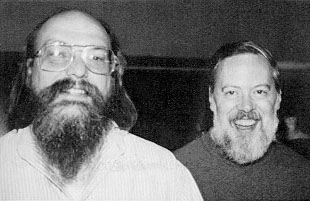
\includegraphics[width=\linewidth]{./gfx/KTDR}
	\caption%
		[Ken Thompson und Dennis Ritchie (1973) -- die Entwickler der Sprache C]
		{Ken Thompson und Dennis Ritchie (1973) -- die Entwickler der Sprache C\newline
		\url{https://en.wikipedia.org/wiki/Dennis_Ritchie}}
	\vspace{-20pt}
\end{wrapfigure}
Bis heute zählt die Sprache C zu einer der bedeutendsten Programmiersprachen. Von der Vielzahl an  Programmierpsprachen, die für verschiedenste Einsatzbereiche zur Verfügung stehen, ist ein Großteil von C beeinflusst. Ungeachtet der Existenz dieser Spezialisierungen bleibt C als Allzweck-Sprache von Bedeutung.

Es ist nicht bekannt, ob die Entwickler \emph{Dennis Ritchie} und \emph{Ken Thompson} bereits die Vision der großen Erfolge hatten, die die Sprache C einmal erreichen würde. Wie die meisten Innovationen sah auch C viele Veränderungen über die Zeit. Vermutlich der größte Erfolg ist die Tatsache, dass C bis in die jüngste Zeit hinein relevant blieb. Für die Entwickler ist es sicherlich sehr erfüllend zu sehen, dass C nicht als überholt oder als nur in Nischenanwendungen nützlich gilt. Stattdessen ist C als starke Allzweck-Sprache anerkannt.

Das Ursprüngliche Ziel der Entwickler war nicht die Entwicklung einer neuen Sprache. Tatsächlich war es erst das Zusammenspiel mehrerer Zufälle, die die Entwicklung der Sprache anstoßen. In den 1960ern arbeitete Dennis Ritchie bei Bell Labs (AT\&T) an einem Betriebssystem das von vielen Anwendern gleichzeitig benutzt werden konnte. Dieses Projekt \emph{MULTICS} (Multiplexed Information and Computer Services) sollte die gemeinsame Verwendung von Rechenressourcen erlauben. Von dem Projekt versprach man sich viele Verbesserungen -- aber bald stellte sich heraus, dass die Kosten für die Umsetzung die Vorteile überwiegen würden. Bell Labs zog sich graduell aus dem Projekt zurück.

Vor diesem Hintergrund schloss sich Ritchie dem Team von Ken Thompson und Brian Kernighan an. Thompson entwickelte in der Sprache Assembler ein Dateisystem für den DEC PDP-7 Supercomputer. Weitere Verbesserungen daran führten schließlich zur Konzeption des Betriebssystems UNIX, in dem einige der Ideen von MULTICS wieder auflebten. Tatsächlich weist schon der Originalname des neuen Projekts -- UNICS (Uniplexed Information and Computing Service) -- auf seine Verwandtschaft mit dem früheren Projekt hin.

UNIX wurde in Assembler geschrieben, was leicht für Computer umzusetzen ist, für Menschen aber eine herausfordernde Arbeitsumgebung darstellt. Um die Arbeit an UNIX zu erleichtern kamen die Sprachen Fortran und B zum Einsatz. Aus den Einschränkungen, die diese Sprachen brachten, erwuchs die Idee für die Sprache C.

Die Sprache B -- eine Weiterentwicklung der Sprache BCPL von Martin Richards -- stellte sich als nützliches Werkzeug in der Entwicklung von UNIX heraus. Jedoch mussten auch hier, wie auch in Assembler, Daten in Maschinensprache zur Verfügung gestellt werden. Datenstrukturen wurden in B ebenfalls nicht unterstützt.

Für die effiziente Fortsetzung der Arbeiten musste sich etwas ändern. Aus diesem Grunde machten sich Ritchie und seine Kollegen in den Jahren 1971 bis 73 daran, die Einschränkungen, die B ihnen auferlegte, abzuschalten. Es sollte nicht vergessen werden, dass die Sprache C im Geiste von B entwickelt wurde -- trotz oder gerade wegen dessen Beschränktheit. Viele Features und Konzepte wurden beibehalten, während neue Ideen -- darunter Datentypen und Strukturen -- hinzugefügt wurden. Der Name C weist direkt darauf hin, dass es sich hierbei um einen Nachfolger der Sprache B handelt. Anfangs wurde C im Hinblick auf die Arbeit an UNIX entwicklet. Um die Performance des Kernels und die Arbeit am Betriebssystem zu verbessern wurden viele UNIX-Komponenten neu in C umgeschrieben.

Ritchie und Kernighan dokumentierten ihr Werk in dem Buch \emph{The C Programming Language}. Obwohl Kernighan behauptete, keinen Einfluss auf das Design der Sprache C genommen zu haben, ist er doch der Autor vieler berühmter UNIX-Programme.

Bald begann C, in PCs für die Software-Entwicklung eingesetzt zu werden. Die erste (kleinere) Änderung am Sprachkonzept fand im Jahr 1983 statt, als das American National Standards Institute (ANSI) ein Kommittee zur Standardisierung der Sprache bildete. Einige Modifikationen wurden vorgenommen, die Code in der nun normierten Sprache kompatibler zu Vorgängerversionen machte. Im Jahre 1989 wurde der neue Standard verabschiedet und ist heute als ANSI C oder C89 bekannt. Die International Organization for Standardization (ISO) trug auch zur Standardisierung von C bei.

Im Laufe der Zeit hat sich C stark weiterentwickelt und Features wie Speichermanagement, Funktionen, Klassen und Bibliotheken in ihren Umfang aufgenommen und wird heute in einigen der größten und bekanntesten Projekte der Welt verwendet. Die Sprache beeinflusste die Entwicklung vieler anderer sprachen wie AMPL, AWK, csh, C++, C--, C\#, Objective-C, Bit C, D, Go, Java, JavaScript, Julia, Limbo, LPC, Perl, PHP, Pike, Processing, Python, Rust, Seed7, Vala und Verilog. 

Sind Sie ein Windows-User? Dann benutzen Sie ein Produkt, das vorwiegend in C geschrieben ist. Dasselbe gilt für MacOS, Linux, Android, iOS als auch für das Windows Phone -- kurz für alle modernen Betriebssysteme. Weiter findet C auch verbreitete Anwendung in Embedded Systems wie sie in Fahrzeugen, Smart TVs und den vielen Elementen des Internet of Things (IoT) verbaut sind.

Die vielfältigen Anwenungsfelder von C sind zu zahlreich, um sie hier aufzulisten. Einige jedoch seien als Beispiel genannt:
\begin{itemize}
\item Entwicklung von Compilern
\item Datenbanken 
\item Computer- und Handy-Spiele
\item Der UNIX-Kernel in seiner fortlaufenden Entwicklung
\item Auswertung Mathematischer Gleichungen
\item Design von Netzwerk-Geräten
\end{itemize}

Wie alle der großen Erfindungen entstand die Sprache C aus einer Notwendigkeit heraus. Die Probleme und Umstände der Zeit ihrer Entwicklung waren die Insporation für die Konzeption der Sprache. Anders als viele Sprachen, die heute als (fast) ausgestorben gelten, \enquote{gedeiht} C auch weiterhin. Einige Sprachen finden heute nur noch in Nischenbereichen Anwendung -- Fortran etwa kommt nur noch im Engineering-Bereich zum Einsatz, und COBOL hat kaum mehr Relevanz. C dagegen ist nicht nur weiterhin eine Sprache, die es zu kennen lohnt. Sie ist und bleibt Einfluss für die Weiterentwicklung bestehender und Konzeption neuer Sprachen. aufwändige Selbst Technologien wie das IoT, AI und Automations-Konzepte konnten sich nicht von der Sprache C lösen. Es bleibt zu erwarten, dass diese Sprache auch lange in die Zukunft ein Teil der Programmier-Welt bleiben wird.
\end{appendices}
